\chapter{Server Side}

\section{REST}
Wir haben RESTlos genug von diesem Thema! REST steht noch immer für Representational State Transfer. Es basiert auf HTTP und ist zustandslos. REST eignet sich gut zum cachen. REST beschreibt letztendlich nur die \emph{korrekte} Verwendung von diversen Technologien:

\begin{itemize}
	\item Generisches Ressourcen-Interface (HTTP-Methoden)
	\item Adress- und Namensgebungen (URI)
	\item Ressourcen-Repräsentationen (HTML, XML, JPG, etc.)
	\item Medientypen (text/html, text/json, etc.)	
\end{itemize}

\emph{Safe Methods} modifzieren eine Ressource nie. GET, HEAD oder OPTIONS dürfen den Status der Ressource nicht verändern. Natürlich manipulieren sie irgendwelche Dinge auf dem Server, wie beispielsweise einen Zähler, aber nicht die Ressource in ihrer Repräsentation. Im Zentrum steht hier der einmalige Aufruf, natürlich ist die Methode auch nach mehreren Aufrufen immer noch \emph{safe}. \emph{Idempotent Methods} sind Methoden, welche x-mal aufgerufen werden können ohne dass jedesmal neue Ressourcen-Repräsentationen entstehen. Mit anderen Worten: Das mehrfache durchführen der genau gleichen Operation ändert die Daten nicht.

\begin{figure}[h!]
\centering
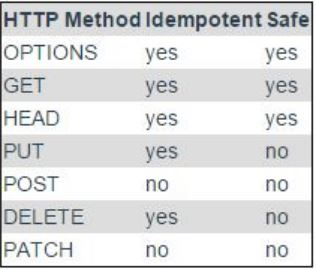
\includegraphics[width=0.5\linewidth]{fig/http-verbs}
\caption{HTTP-Verbs}
\label{fig:http-verbs}
\end{figure}

\begin{figure}[h!]
\centering
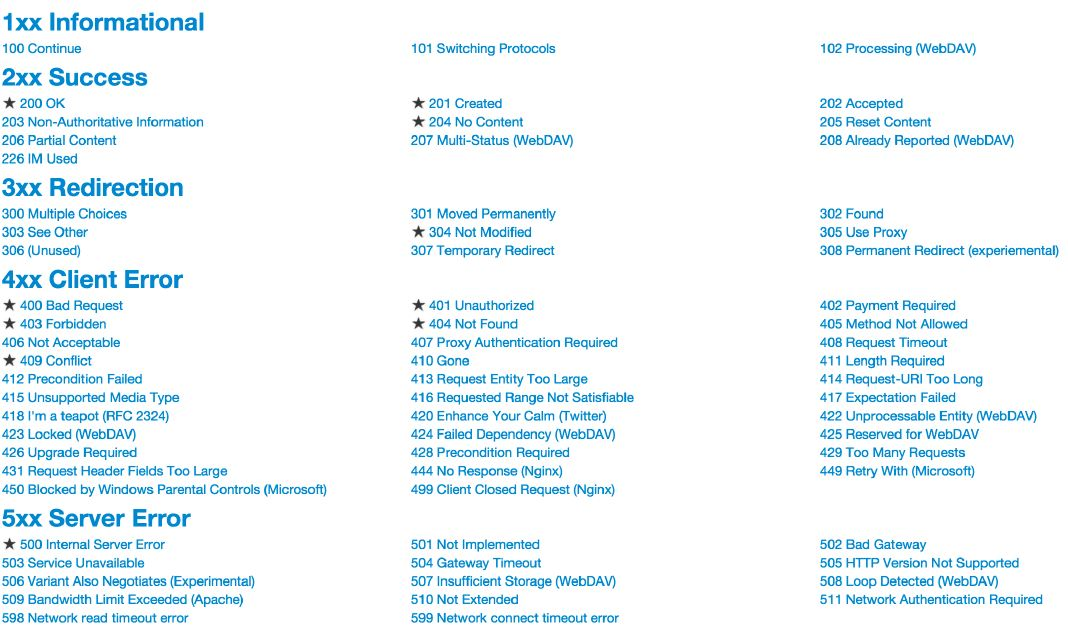
\includegraphics[width=1\linewidth]{fig/http-statuscodes}
\caption{HTTP-Statuscodes}
\label{fig:http-statuscodes}
\end{figure}

Wir unterscheiden zwischen \emph{Collection Resources} (../Resource)  und \emph{Element Resources} (../Resource/123).

\begin{figure}[h!]
\centering
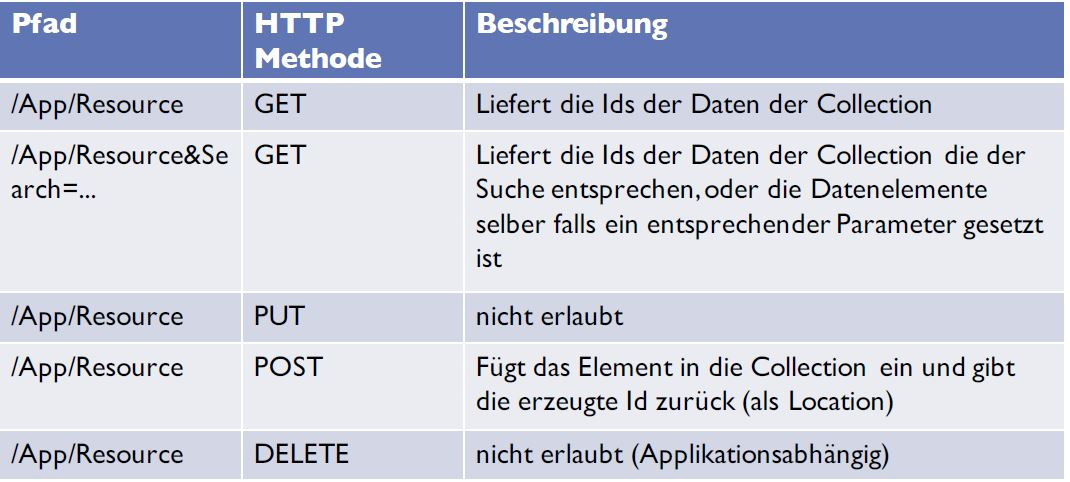
\includegraphics[width=0.7\linewidth]{fig/rest-collection-interface}
\caption{Collection-Interface}
\label{fig:rest-collection-interface}
\end{figure}

\begin{figure}[h!]
\centering
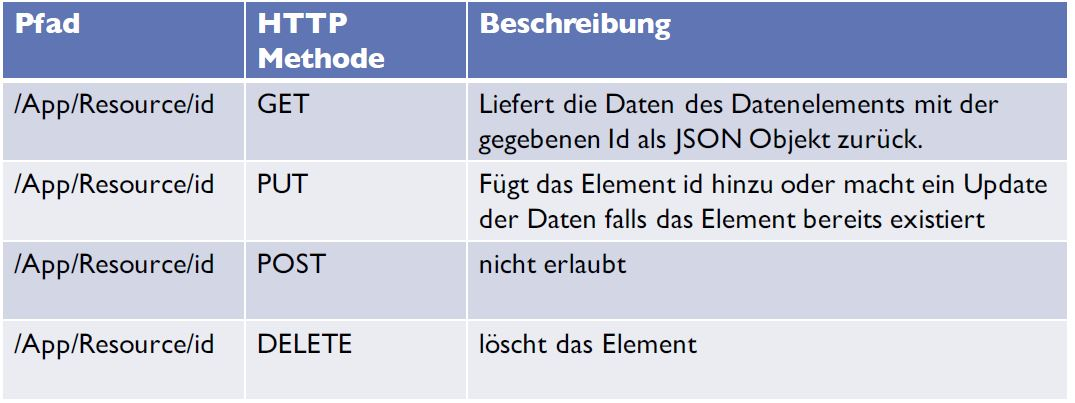
\includegraphics[width=0.7\linewidth]{fig/rest-element-interface}
\caption{Element-Interface}
\label{fig:rest-element-interface}
\end{figure}
